\documentclass[11pt,a4paper]{article}

\usepackage[margin=2.4cm]{geometry}
\usepackage{amsmath,amssymb}
\usepackage{graphicx}
\usepackage{booktabs}
\usepackage{caption}
\usepackage{xcolor}
\definecolor{linkblue}{RGB}{30,60,140}
\usepackage[colorlinks=true,linkcolor=linkblue,citecolor=linkblue,urlcolor=linkblue]{hyperref}
\usepackage{microtype}

\graphicspath{{../results/figures/}}
\captionsetup{font=small,labelfont=bf}

\title{Optimal Athletic Programming in Triathlon\\
       using Linear and Integer Programming}
\author{Emmanouil Vichos (AM 1100830)\\[2pt]
        \small Linear and Combinatorial Optimization --- University of Patras\\
        \small Supervisor: Prof.\ S.\ Daskalaki}
\date{\today}

\begin{document}
\maketitle

\begin{abstract}
Triathlon combines swimming, cycling and running, and its triple nature generates
three interconnected decision problems: how to allocate training load, which races
to enter, and how to pace a race. This project models all three with Linear
Programming (LP) and 0--1 Mixed-Integer Programming (MIP), using fifteen months of
the author's real training data (574 activities from a Strava export). The models
form a pipeline: the fitness state produced by the training model gates race
selection and sets the energy budget for pacing. Beyond the base solutions, the
project exercises the full course syllabus --- Simplex-based LP solving, duality and
shadow-price interpretation, right-hand-side ranging, Branch \& Bound with LP
relaxation gaps, and a network-flow reduction with an empirical total-unimodularity
demonstration. Several optimal solutions reproduce established coaching wisdom
(build-then-taper periodization, ``steady bike, hard run'' pacing) without it being
imposed, while sensitivity analysis reveals which recommendations are driven by the
objective and which by the constraints.
\end{abstract}

\section{Introduction and Motivation}

A competitive age-group triathlete faces three planning problems at different time
scales. Over a macrocycle of 12--20 weeks they must decide how many hours to train
in each sport and at which intensity, trading fitness gains against accumulated
fatigue. Over a season they must choose a race calendar under a money budget,
limited days off work, and physiological recovery requirements. Finally, on race
day they must distribute a limited energy reserve across three consecutive legs to
minimize finishing time.

These problems are usually solved by rules of thumb. This project instead treats
them as mathematical programs and asks what an optimizer would do: Model~1 is an
LP that allocates weekly training load; Model~2 is a 0--1 MIP that selects the race
calendar; Model~3 is an LP that computes a pacing strategy. The three are coupled
sequentially: Model~1's terminal fitness state is a readiness gate in Model~2 and
determines the energy budget in Model~3
(Fig.~\ref{fig:pipeline}).

\begin{figure}[h]
\centering
\begin{tabular}{ccccc}
\textbf{Model 1 (LP)} & $\longrightarrow$ & \textbf{Model 2 (0--1 MIP)} & $\longrightarrow$ & \textbf{Model 3 (LP)}\\
training load & & race calendar & & pacing strategy\\
\emph{fitness state} & & \emph{which races?} & & \emph{how to race?}
\end{tabular}
\caption{The three-model pipeline. Arrows carry the CTL/ATL fitness state.}
\label{fig:pipeline}
\end{figure}

Two features distinguish the project from a textbook exercise. First, all inputs of
Model~1 are estimated from the author's real training history; the numbers below
are personal, not stylized. Second, each model is accompanied by the analysis the
course emphasizes: duals and their physiological meaning, value functions under
RHS variation, integrality gaps, and alternative optima.

\section{Literature}

The training model rests on the fitness--fatigue framework of Banister et
al.~\cite{banister1975}, applied to triathletes by Millet et
al.~\cite{millet2002} and revisited critically by Hellard et
al.~\cite{hellard2006}; taper practice follows Mujika~\cite{mujika2009}, and a
recent optimization treatment of tapering appears in Ceddia et
al.~\cite{ceddia2025}. Race selection is a knapsack-type selection problem in the
tradition of integer-programming modeling~\cite{nemhauser1988,williams2013}; sports
scheduling as an IP application area is surveyed by Ribeiro~\cite{ribeiro2012} and
advocated pedagogically by Trick~\cite{trick2005}. Pacing strategy in endurance
sport is reviewed by Abbiss and Laursen~\cite{abbiss2008}; the physiological
asymmetries between cycling and running that motivate our coupling constraint are
documented by Millet et al.~\cite{millet2009} and factors specific to triathlon
pacing by Wu et al.~\cite{wu2014}; a numerical-optimization approach to pacing
appears in Ni et al.~\cite{ni2022}. General LP/OR background follows Dantzig
\cite{dantzig1963} and Hillier--Lieberman~\cite{hillier2015}.

\section{Data}

The data pipeline processes the author's Strava bulk export: 598 activities from
October 2023 to June 2026, of which 574 swim/bike/run sessions are kept. Each
activity contributes date, sport, moving time, average heart rate (HR) and, for
cycling, average power. For every activity a Banister training impulse is computed,
\[
\text{TRIMP} \;=\; t \,\cdot\, \text{HRr} \cdot 0.64\, e^{1.92\,\text{HRr}},
\qquad
\text{HRr} = \frac{\text{HR} - \text{HR}_{\text{rest}}}{\text{HR}_{\max} - \text{HR}_{\text{rest}}},
\]
with $t$ in minutes. The 125 activities without HR (mostly older runs) receive a
sport-specific default intensity. Daily loads are smoothed exponentially into a
chronic training load (CTL, $\tau = 42$ days) and an acute training load (ATL,
$\tau = 7$ days); the balance $\text{TSB} = \text{CTL} - \text{ATL}$ measures
freshness. At the time of the study the athlete's state was
$\text{CTL}_0 = 78.1$, $\text{ATL}_0 = 91.5$, $\text{TSB} = -13.4$: solid fitness,
currently fatigued.

Each activity is also classified into an intensity bucket --- easy (Z1--2), moderate
(Z3), hard (Z4+) --- relative to a \emph{sport-specific} lactate-threshold HR (run
173, bike 166, swim 164 bpm), since HR reads systematically lower in cycling and
swimming at equal effort. The TRIMP-per-hour rates $r_{db}$ by (sport, bucket) that
parameterize Model~1 are estimated from the data where at least five activities
exist and from the Banister formula at the bucket's representative HR otherwise
(4 of 9 cells, flagged as theoretical).

\begin{table}[h]
\centering\small
\begin{tabular}{lrrr}
\toprule
TRIMP/hour & easy (Z1--2) & moderate (Z3) & hard (Z4+)\\
\midrule
swim & 43.5 & $94.1^{\ast}$ & $136.6^{\ast}$\\
bike & 68.3 & 86.9 & $142.7^{\ast}$\\
run  & 81.6 & 102.8 & $166.0^{\ast}$\\
\bottomrule
\end{tabular}
\caption{Estimated load rates $r_{db}$. Starred cells have fewer than five
observed activities and use the theoretical Banister rate at the bucket's
representative heart rate.}
\label{tab:rates}
\end{table}

Candidate races for Model~2 are a constructed but documented dataset of 17 events
(Greek domestic, European, and long-haul; entry fees at official price ranges,
travel costs and vacation-day requirements by destination), with deliberate
structural features: same-weekend conflicts, a championship pair two weeks apart,
and a high-value early-season race the athlete cannot be fit for. All assumptions
are recorded in the repository (\texttt{docs/race\_data\_assumptions.md}).

\section{Model 1 --- Optimal Training-Load Allocation (LP)}

\subsection{Formulation}

For disciplines $D=\{\text{swim},\text{bike},\text{run}\}$, buckets
$B=\{\text{easy},\text{mod},\text{hard}\}$ and weeks $W=\{1,\dots,T\}$ ($T=16$ for
an Olympic-distance goal), the decision variables are training hours
$h_{dbw}\ge 0$ ($3\times3\times16 = 144$ variables). Weekly load and the Banister
recursion enter as equality-defined auxiliaries, keeping the model an LP:
\begin{align*}
L_w &= \sum_{d,b} r_{db}\, h_{dbw},\\
\text{CTL}_w &= \lambda_c\, \text{CTL}_{w-1} + (1-\lambda_c)\,\tfrac{L_w}{7},
&\lambda_c &= e^{-7/42},\\
\text{ATL}_w &= \lambda_a\, \text{ATL}_{w-1} + (1-\lambda_a)\,\tfrac{L_w}{7},
&\lambda_a &= e^{-7/7}.
\end{align*}
The objective maximizes predicted race-day performance in the Banister sense,
\[
\max\; p_T = k_1\,\text{CTL}_T - k_2\,\text{ATL}_T, \qquad (k_1,k_2)=(1,2).
\]
Maximizing TSB alone would be degenerate (the optimum would be to rest);
the Banister form rewards early CTL accumulation, whose contribution persists,
while early-week ATL decays away by race day. The constraints, for every week $w$:
\begin{align}
\sum_{d,b} h_{dbw} &\le H^{\max}_w
    && \text{phase-dependent hours ceiling (12\,h baseline)}\\
h^{\min}_d \le \sum_{b} h_{dbw} &\le h^{\max}_d \quad \forall d
    && \text{discipline bounds (pool access, injury risk)}\\
\sum_{d} \left(h_{d,\text{mod},w} + h_{d,\text{hard},w}\right)
    &\le 0.2 \sum_{d,b} h_{dbw}
    && \text{80/20 polarized-training rule}\\
\text{ATL}_w &\le 110
    && \text{overtraining guard}\\
L_w &\le 1.1\, L_{w-1}
    && \text{ramp-rate limit } (w \ge 2)\\
L_w &\le \theta_w\, \bar{L}_{\text{build}} \quad w \in \text{taper}
    && \theta_{15} = 0.6,\; \theta_{16} = 0.4
\end{align}
where $\bar{L}_{\text{build}}$ is the (linear) average build-phase load. The solved
LP has 192 variables and 209 constraints.

\subsection{Results}

\begin{figure}[t]
\centering
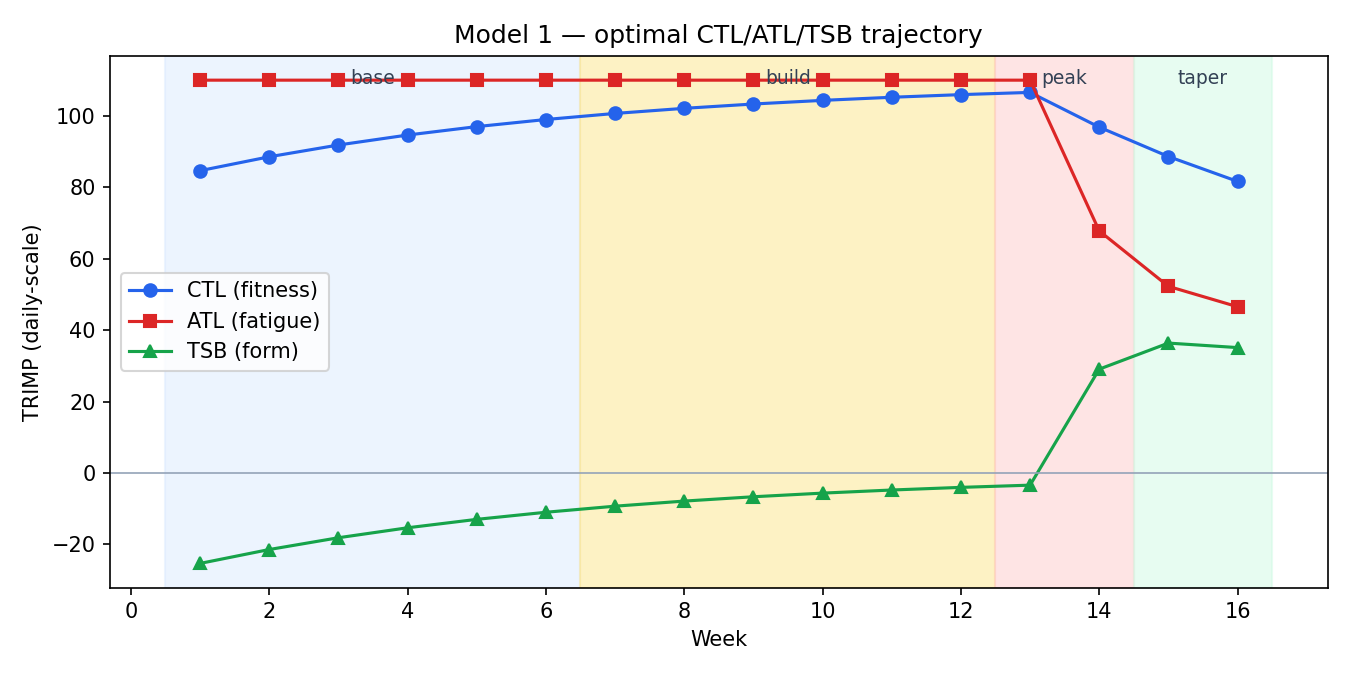
\includegraphics[width=.85\textwidth]{model1_trajectory.png}
\caption{Optimal CTL/ATL/TSB trajectory. The plan rides the fatigue ceiling
($\text{ATL}=110$) for 13 weeks, building CTL from 78 to 107, then tapers.}
\label{fig:m1traj}
\end{figure}

The optimal plan (Fig.~\ref{fig:m1traj}) holds weekly load exactly at the value
that keeps ATL on its ceiling for 13 weeks --- the fatigue constraint, not available
time, is binding --- and then cuts volume to one third for the final three weeks,
arriving at race day with $\text{CTL}=81.6$, $\text{ATL}=46.5$,
$\text{TSB}=+35$. Notably, only weeks 15--16 are \emph{constrained} to taper; the
optimizer starts tapering in week 14 by choice. Build-then-peak-then-taper
periodization is thus a \emph{property of the optimum}, not an assumption. The
weekly discipline allocation (Fig.~\ref{fig:m1hours}) keeps all three sports within
realistic bounds while the intensity mix sits exactly on the 80/20 polarization
constraint --- the coaching rule is recovered as a binding constraint of the
optimal plan.

\begin{figure}[t]
\centering
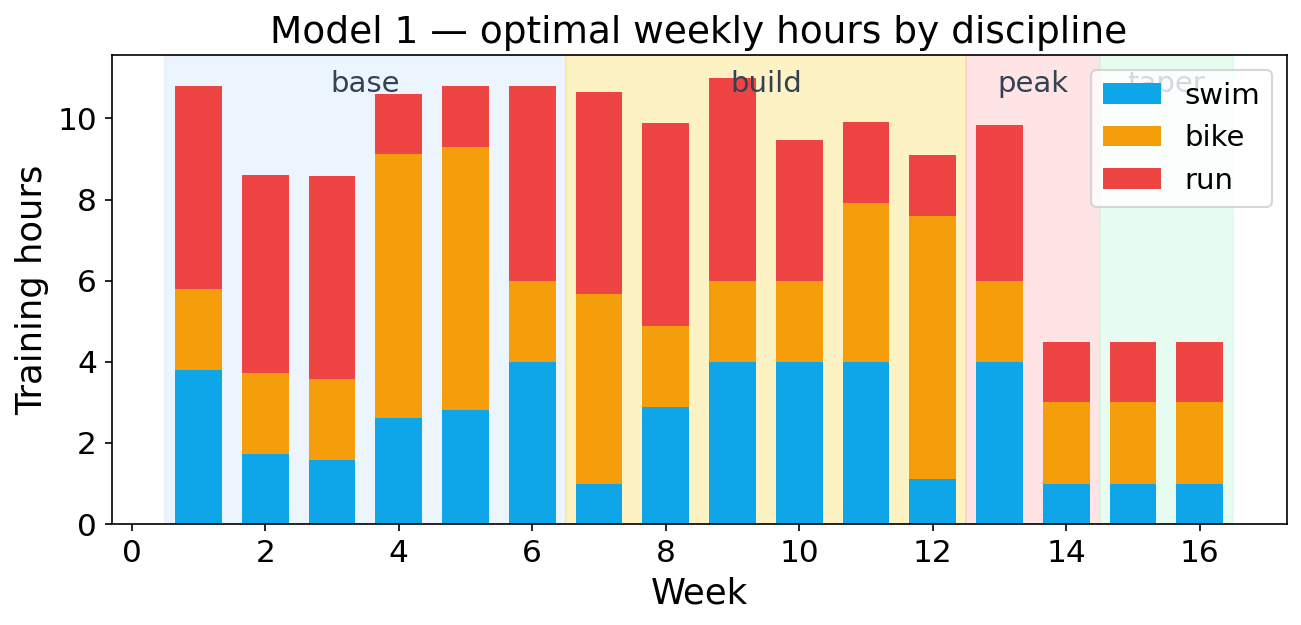
\includegraphics[width=.85\textwidth]{model1_weekly_hours.png}
\caption{Optimal weekly training hours by discipline across macrocycle phases.}
\label{fig:m1hours}
\end{figure}

\subsection{Duality and sensitivity}

\paragraph{RHS ranging.} Re-solving for hour ceilings $H^{\max}\in[8,16]$ traces
the LP value function (Fig.~\ref{fig:m1rhs}): empirically piecewise-linear and
concave, with slopes $1.55 \to 0.94 \to 0.12 \to 0.06 \to 0$. Below
$8.5$\,h the model is infeasible (discipline minimums collide with taper caps);
above $10.5$\,h extra hours are worthless because the ATL ceiling binds first. For
this athlete, recovery capacity --- not free time --- limits performance.

\begin{figure}[t]
\centering
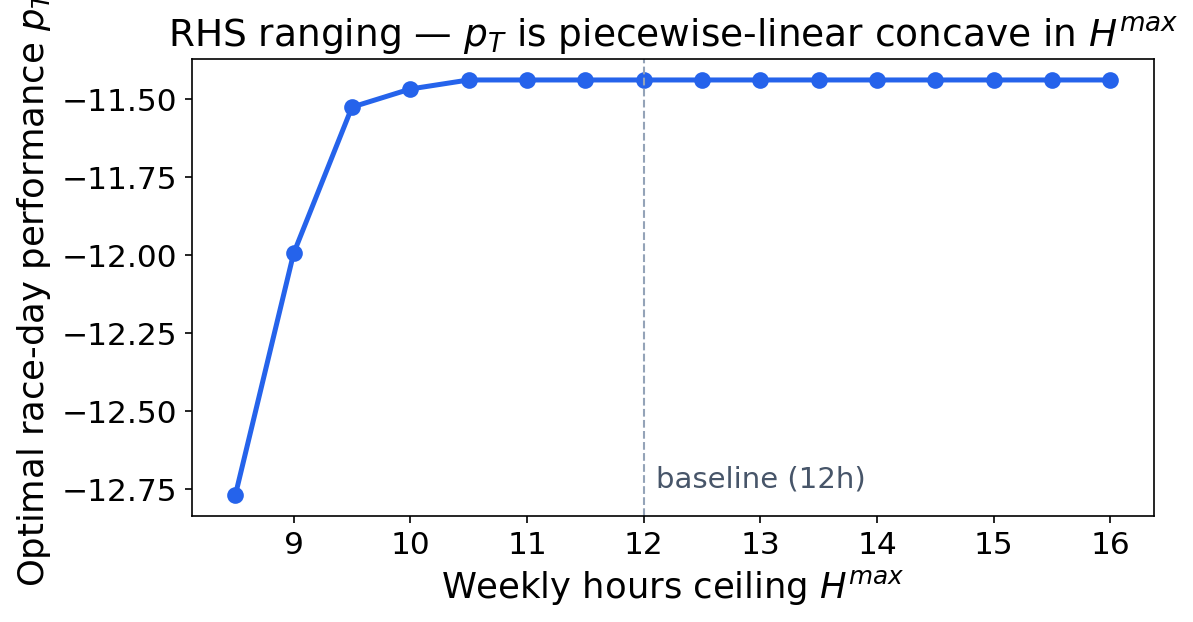
\includegraphics[width=.7\textwidth]{model1_rhs_ranging.png}
\caption{Value function of the weekly-hours RHS: piecewise-linear, concave,
saturating at 10.5\,h/week.}
\label{fig:m1rhs}
\end{figure}

\paragraph{Shadow prices.} The largest duals in absolute value belong to the
race-week discipline minimums: a forced hour of running in week 16 costs $12.9$
performance points --- the model would rather rest completely. The ATL-ceiling duals
peak in late build (week 12: $+0.07$ per TRIMP/day of extra fatigue tolerance),
quantifying the value of recovery capacity when it matters most.

\paragraph{Alternative optima.} Fixing the objective at $p^\ast$ and re-solving
with total season hours as a secondary objective yields plans from 124.2\,h to
162.3\,h at \emph{identical} performance: the optimal face has positive dimension,
and the same race-day form is achievable with 38 fewer training hours. Practically,
the efficient (minimum-hours) plan is preferable; theoretically, this is LP
degeneracy made visible. Realistic per-discipline weekly caps were added to bound
this degeneracy for the reported plan.

\paragraph{Benchmark against a coaching heuristic.} A standard
``fill the available hours, 20/45/35 discipline split, 80/15/5 intensity split''
plan violates the ATL ceiling in 13 of 16 weeks and scores $p_T=-69.5$ versus the
optimum $-11.4$. The heuristic does, however, arrive at race day with
$\text{TSB}=+21$, inside the band $+15\ldots+25$ recommended by coaching practice,
while the LP over-tapers to $+35$ --- see the $k_2$ discussion in
Section~\ref{sec:sensitivity}.

\section{Model 2 --- Race-Calendar Selection (0--1 MIP)}

\subsection{Formulation}

For candidate races $i \in R$ with week $t_i$ and distance class $c_i$, binary
variables $x_i$ select the season calendar. The risk-adjusted value of a race is
\[
v_i = q_i\left(\alpha\,\text{pts}_i + \beta\,\text{strat}_i
      + \gamma\,\text{enj}_i + \varphi\,\text{fit}_i\right),
\]
where $q_i$ is the probability of good race-day weather, enjoyment
$\text{enj}_i$ aggregates subjective organization/scenery/swim scores, and
suitability $\text{fit}_i$ is computed from \emph{objective} course data ---
elevation gain per km per leg matched to the athlete's flat-course preference. The
program is a two-dimensional knapsack with temporal side constraints:
\[
\max \sum_i v_i x_i
\quad\text{s.t.}\quad
\sum_i \kappa_i x_i \le 2500 \text{ EUR}, \qquad
\sum_i \delta_i x_i \le 12 \text{ days},
\]
at most two races per month; recovery spacing
$x_i + x_j \le 1$ for pairs closer than the recovery requirement of the earlier
race (sprint 1, Olympic 2, 70.3 4 weeks); at least one championship-quality
``A-race''; and a readiness gate from Model~1 --- a projected season CTL curve
(off-season start, load ramping to Model~1's build level) must reach a
class-specific requirement by race week, which excludes the high-value but
too-early Dubai 70.3.

\subsection{Results}

The optimum selects 8 of 17 races for a value of 571.7
(Table~\ref{tab:calendar}, Fig.~\ref{fig:m2cal}), spending 2250 of 2500 EUR
and 11 of 12 vacation days --- both knapsack dimensions are nearly binding. The
recovery constraint forces a choice between the National Championship and the
home-soil 70.3 two weeks later; the optimizer picks the 70.3. The LP relaxation
scores 600.5, an integrality gap of $5.0\%$, with eight fractional variables
including the championship conflict split exactly $0.5/0.5$ --- a textbook
illustration of why Branch \& Bound is needed. At the relaxation's optimum the
budget dual is $0.094$ value/EUR while the vacation-days dual is
$\approx 0$: at the baseline, money, not time off, is the scarce resource.

\begin{table}[h]
\centering\small
\begin{tabular}{llllrr}
\toprule
& Race & Date & Class & Cost (EUR) & Value\\
\midrule
R01 & TRIMORE Athens Sprint & Mar 14 & sprint & 45 & 45.1\\
R02 & Challenge Heraklion & Apr 18 & olympic & 290 & 83.8\\
R03 & TRIMORE Syros & May 9 & olympic & 210 & 56.6\\
R05 & Athens Riviera & Jun 6 & olympic & 60 & 69.1\\
R07 & Thessaloniki Sprint & Jun 27 & sprint & 160 & 46.6\\
R09 & Nafplio & Jul 18 & olympic & 135 & 48.0\\
R11 & Ironman 70.3 Budapest & Aug 22 & 70.3 & 770 & 104.7\\
R14 & Ironman 70.3 Costa Navarino & Sep 26 & 70.3 & 580 & 117.7\\
\bottomrule
\end{tabular}
\caption{Optimal 2027 race calendar (A-race: Costa Navarino).}
\label{tab:calendar}
\end{table}

\begin{figure}[t]
\centering
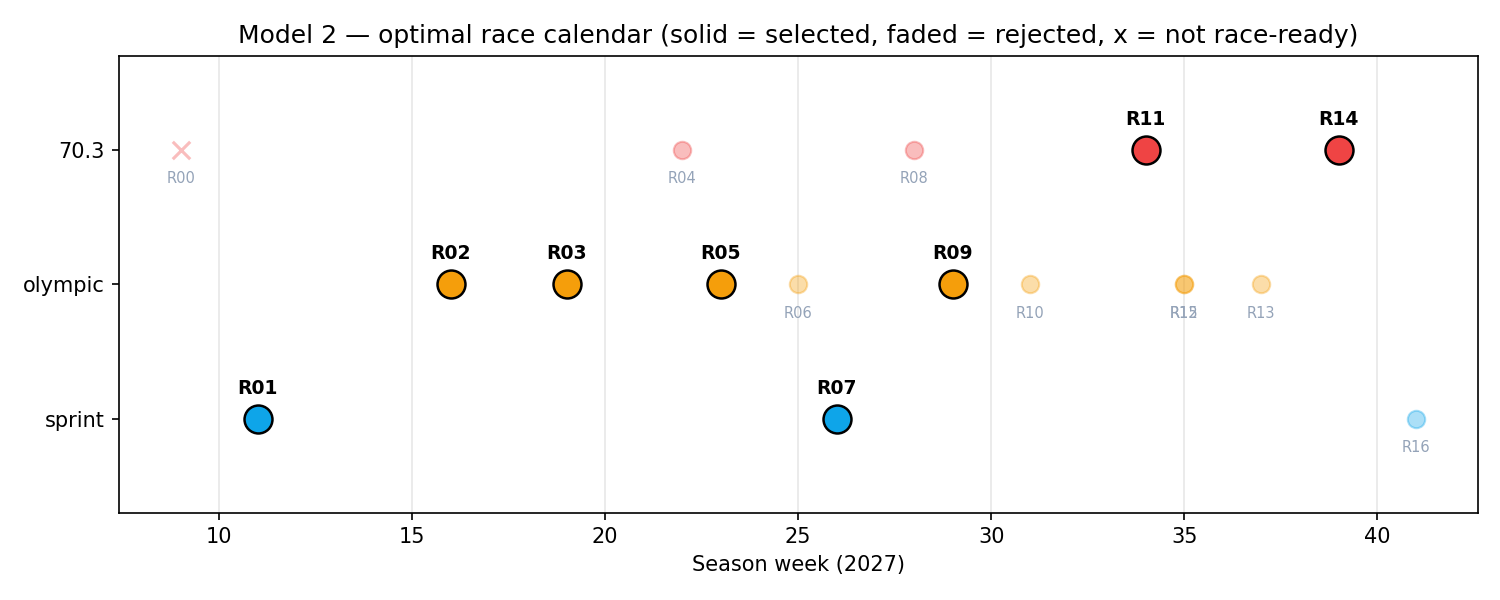
\includegraphics[width=.9\textwidth]{model2_calendar.png}
\caption{Season timeline: selected races (solid), rejected (faded),
not race-ready ($\times$).}
\label{fig:m2cal}
\end{figure}

\begin{figure}[t]
\centering
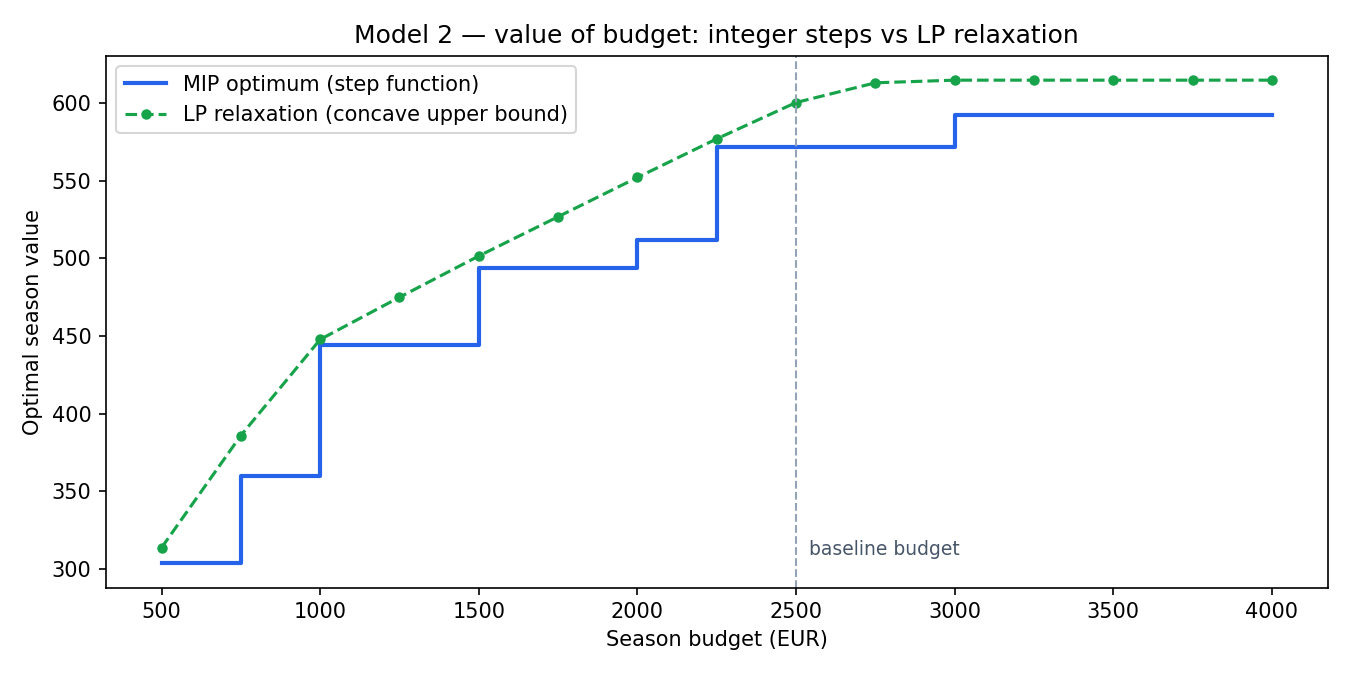
\includegraphics[width=.8\textwidth]{model2_budget_sweep.png}
\caption{Season value vs.\ budget: the MIP optimum is a step function; the LP
relaxation is a concave upper bound. Beyond 3000 EUR the vacation-days budget
becomes binding and money stops mattering.}
\label{fig:m2budget}
\end{figure}

\paragraph{Budget sweep.} Varying the money budget from 500 to 4000 EUR
(Fig.~\ref{fig:m2budget}) shows the characteristic IP behavior: the optimal value
increases in \emph{steps} (races are indivisible) beneath the concave LP-relaxation
curve. Above 3000 EUR the value saturates at 592.7 because all 12 vacation days are
consumed --- the binding constraint switches dimension.

\subsection{Network-flow extension}

Dropping the two knapsacks, the monthly cap and the A-race constraint leaves only
recovery spacing, and the problem becomes a \emph{longest path in a DAG}: nodes are
race-ready races in week order, an arc $i \to j$ exists when the gap respects the
recovery of race $i$, and node weights are the $v_i$. Recovery requirements
compose along chains, so feasible calendars and $S$--$T$ paths coincide. Three
methods were implemented and agree exactly ($z = 639.4$): dynamic programming in
topological order; a flow LP with \emph{continuous} variables; and the restricted
MIP. The flow LP returns an integral solution without any integrality constraints
--- its constraint matrix is a network matrix, hence totally unimodular. The
knapsack constraints are therefore precisely what breaks the network structure and
forces Branch \& Bound in the full model.

\section{Model 3 --- Race Pacing Strategy (LP)}

\subsection{Formulation}

For legs $\Lambda$ and intensity zones $Z1$--$Z5$, the variables $t_{\ell z}\ge 0$
are minutes in zone $z$ during leg $\ell$. Within a zone, speed and metabolic rate
are constants, linearizing the nonlinear speed--energy curve: bike speed scales
with the cube root of power (aerodynamic drag), $v_z = v_{\text{FTP}}
(P_z/\text{FTP})^{1/3}$ with $\text{FTP}=260$\,W; swim/run speeds are fractions of
threshold pace; energy cost per km rises with intensity (economy factors
0.95--1.20). The program minimizes total time subject to covering each leg's
distance, an overall energy budget $E^{\text{tot}} = k_E\cdot\text{CTL}_T$ linked
to Model~1, per-leg caps on time at Z4--Z5, and a bike$\to$run coupling: each kJ of
hard bike work reduces effective run coverage by $\varphi$ km.

\subsection{Results}

\begin{figure}[t]
\centering
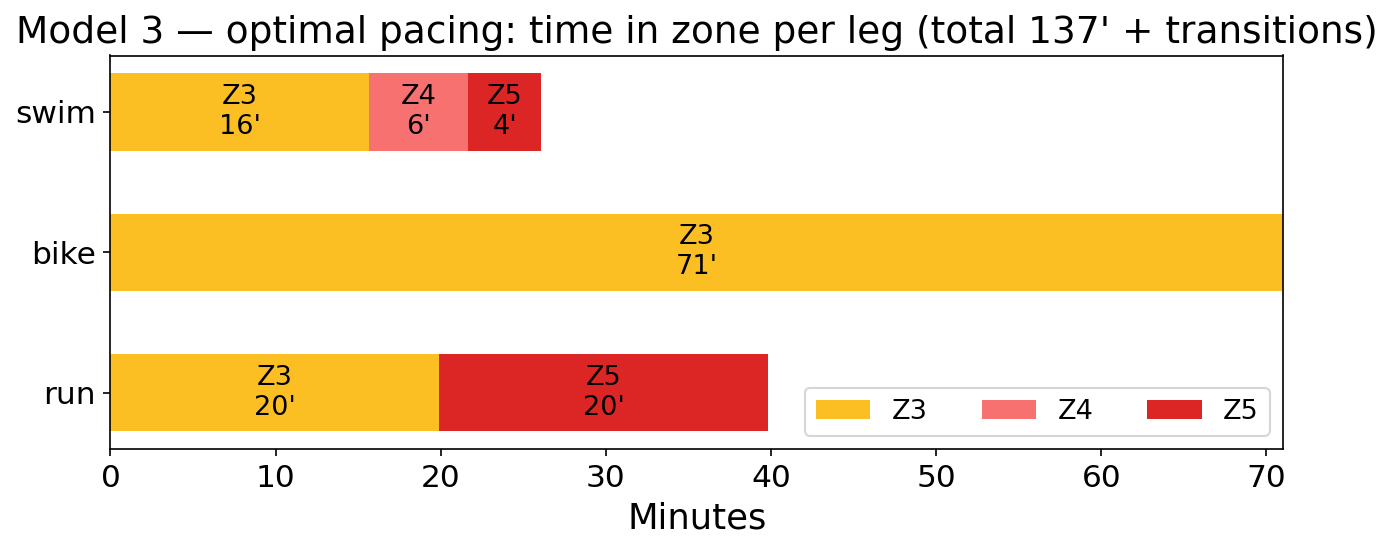
\includegraphics[width=.8\textwidth]{model3_pacing.png}
\caption{Optimal pacing for the Olympic distance: steady Z3 bike, hard run.
Total 140.4 min including transitions; energy budget exactly exhausted.}
\label{fig:m3pacing}
\end{figure}

The optimal Olympic-distance race takes 140.4 minutes: swim 26.1 (mixed Z3--Z5 at
the intensity cap), bike 71.0 entirely at Z3 (33.8 km/h), run 39.8 (half Z3, half
Z5 at the cap), with the 9389 kJ energy budget exactly binding
(Fig.~\ref{fig:m3pacing}). The optimizer \emph{derives} the standard triathlon
advice --- ride steady, run hard: hard biking buys little speed (cube-root curve)
while draining both the shared energy budget and run capacity through the coupling
term.

\subsection{Duality: what is a watt worth?}

The duals answer athlete questions directly. The energy dual is $-0.0071$ min/kJ:
one extra kJ of aerobic capacity saves $0.43$ s. The distance duals price each km:
an extra swim km would cost 26.4 min, bike 2.5, run 6.3. Parametric re-solving over
FTP (Fig.~\ref{fig:m3sweeps}, left) shows each watt below the current 260\,W is
worth $\approx 6$ s, but the marginal value collapses at 260--270\,W: with a fixed
energy budget, more power cannot be fueled. The CTL sweep (right) confirms the
flip side: one CTL point is worth 69--84 s up to $\text{CTL}\approx 85$, then
saturates when speed caps bind instead. For this athlete the data-driven advice is
unambiguous --- build endurance, not peak power.

\begin{figure}[t]
\centering
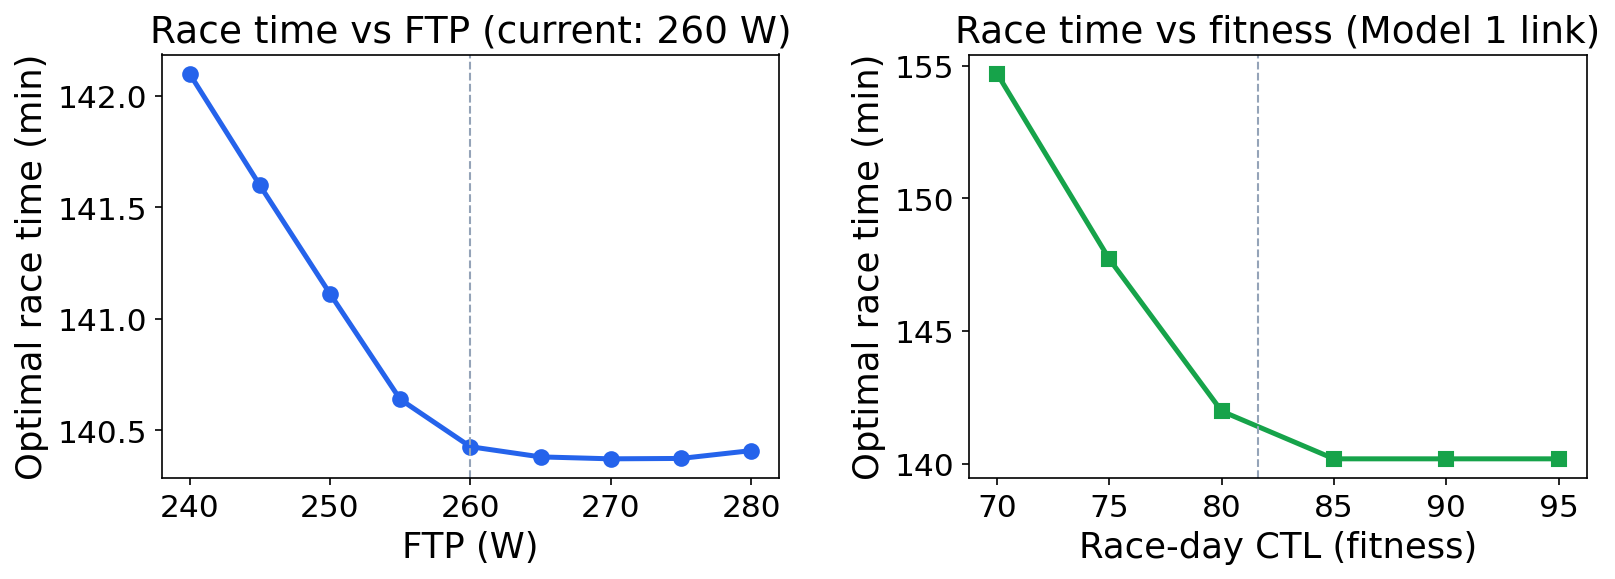
\includegraphics[width=.95\textwidth]{model3_sweeps.png}
\caption{Parametric analysis of Model 3. Left: race time vs.\ FTP --- watts are
worth $\sim$6 s each below 260 W and almost nothing above. Right: race time vs.\
race-day CTL --- fitness is the binding resource up to CTL $\approx 85$.}
\label{fig:m3sweeps}
\end{figure}

\section{Cross-Model Sensitivity Analysis}
\label{sec:sensitivity}

\paragraph{Problem size (distance scenarios).} Re-solving Model~1 for Sprint
(12 weeks, 10\,h ceiling), Olympic (16, 12\,h) and 70.3 (20, 14\,h) scales the LP
from 144 to 240 variables. Longer horizons monotonically improve race-day
performance ($p_T$: $-13.5 \to -11.4 \to -10.4$) --- more weeks allow CTL to be
built early and cheaply --- while the optimal structure (ceiling-riding build, deep
taper, TSB $+33\ldots+36$) is invariant (Fig.~\ref{fig:distance}).

\begin{figure}[t]
\centering
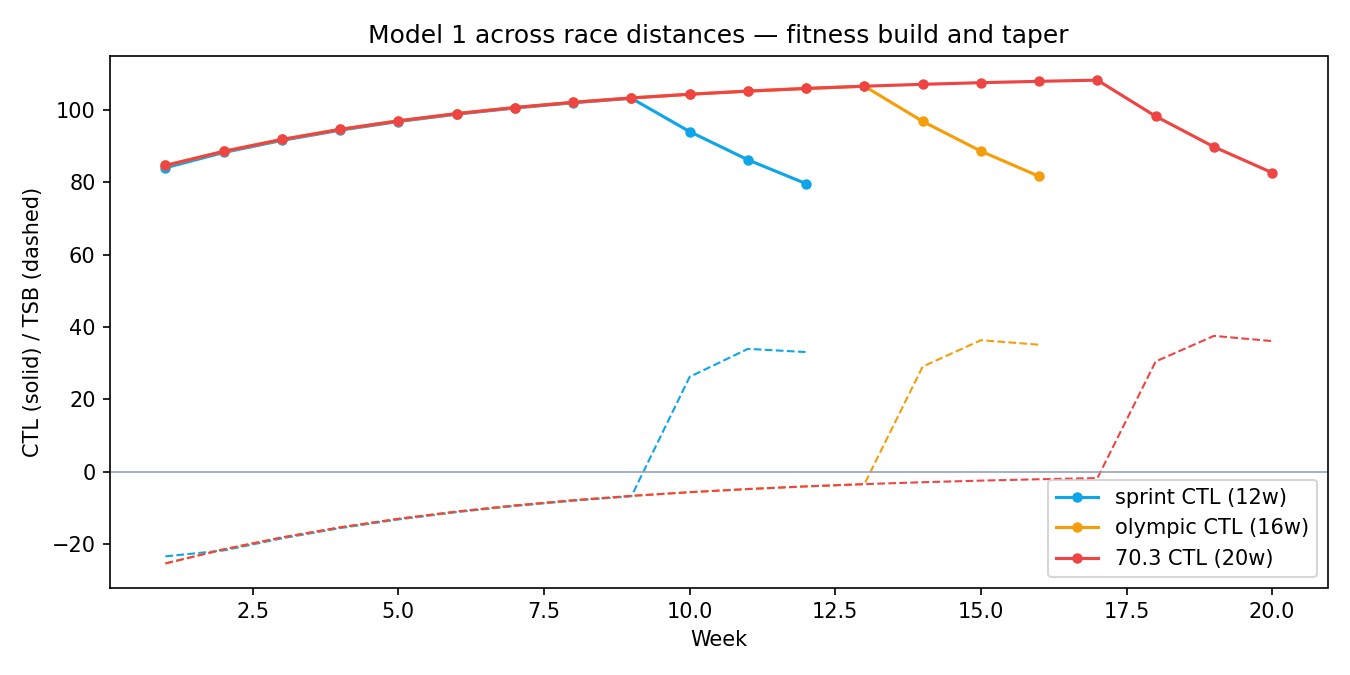
\includegraphics[width=.8\textwidth]{model1_distance_scenarios.png}
\caption{Model 1 across race distances: CTL build (solid) and TSB (dashed) for
12/16/20-week horizons. The build--taper structure is invariant.}
\label{fig:distance}
\end{figure} All instances solve in under 10\,ms with
CBC (Table~\ref{tab:sizes}), whose LP engine is the (dual) Simplex algorithm; the
Simplex method is thus exercised implicitly by every solve in the project.

\begin{table}[h]
\centering\small
\begin{tabular}{lcccc}
\toprule
Model & Type & Variables & Constraints & Solve time\\
\midrule
Model 1 (training) & LP & 192 & 209 & 5 ms\\
Model 2 (calendar) & 0--1 MIP & 17 & 27 & 5 ms\\
Model 3 (pacing) & LP & 15 & 7 & 1 ms\\
\bottomrule
\end{tabular}
\caption{Model sizes and CBC solve times (baseline instances).}
\label{tab:sizes}
\end{table}

\paragraph{Fatigue weight $k_2$.} Sweeping $k_2 \in [1,3]$ barely moves race-day
TSB ($35 \pm 2$): taper depth turns out to be pinned by the \emph{constraints}
(race-week discipline minimums), not by the objective. This is a reassuring
robustness result --- the plan does not hinge on an unmeasurable parameter --- and it
locates the earlier over-taper observation ($+35$ vs.\ the $+15\ldots+25$ coaching
band) in the constraint set: relaxing race-week minimums, not retuning $k_2$,
would close that gap (Fig.~\ref{fig:k2}).

\begin{figure}[h]
\centering
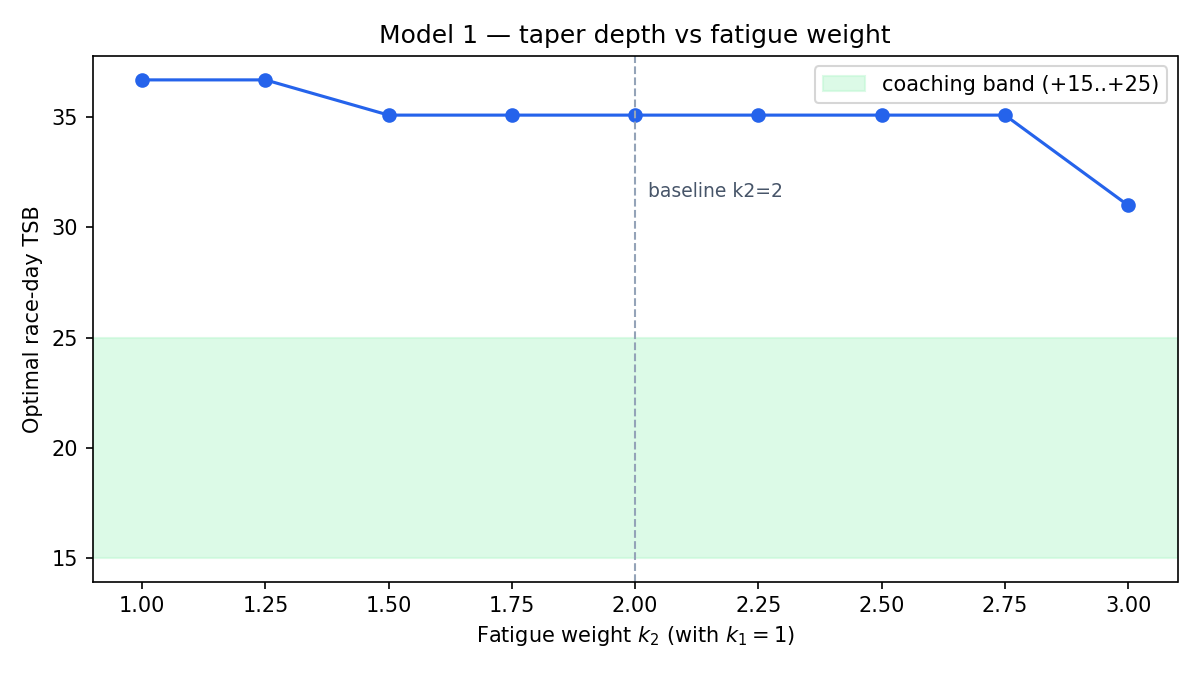
\includegraphics[width=.65\textwidth]{model1_k2_sensitivity.png}
\caption{Race-day TSB vs.\ fatigue weight $k_2$: nearly flat --- taper depth is
constraint-determined, robust to the objective's calibration.}
\label{fig:k2}
\end{figure}

\section{Discussion and Limitations}

Three modeling limitations deserve honesty. First, the weekly Banister recursion
is a coarse time step; daily dynamics would shift constants slightly, though not
the structure of the optimum. Second, the pipeline is sequential rather than
jointly optimal: Model~1's plan is fixed before Model~2 selects races, whereas a
joint model would co-optimize the macrocycle with the calendar (a substantially
larger MIP --- a natural extension). Third, several Model~2/3 parameters
(race values, zone speeds, the energy--CTL constant $k_E$) are constructed from
documented assumptions rather than measured; the sensitivity analyses show which
conclusions survive parameter perturbation. The relay variant mentioned in the
proposal was scoped out in favor of depth (duality, network flows) over breadth.

Against these caveats stand results with practical content: periodization and
``steady bike, hard run'' emerge as optimal rather than assumed; shadow prices
translate into athlete-meaningful quantities (seconds per watt, per kJ, per
vacation day); and the analysis exposes which coaching rules are near-optimal (the
80/20 intensity split) and which are not (filling all available hours).

\section{Conclusions}

The project delivers three coupled optimization models solved on real personal
training data, together spanning the course syllabus: LP modeling and Simplex
solving (Models~1, 3), duality and sensitivity analysis (shadow prices, RHS
ranging, parametric sweeps), integer programming with Branch \& Bound and
integrality-gap analysis (Model~2), and network flows with total unimodularity
(the longest-path reduction). The optimizer independently reproduces core
endurance-coaching principles and, through its dual variables, prices the
athlete's true bottlenecks: recovery capacity in training, money in race
selection, and aerobic endurance --- not peak power --- on race day. All code, data
assumptions and results are reproducible with a single command from the public
repository.\footnote{\url{https://github.com/manos1503/triathlon-optimization}}

\begin{thebibliography}{99}\small

\bibitem{banister1975} E.\,W. Banister, T.\,W. Calvert, M.\,V. Savage, T. Bach,
``A systems model of training for athletic performance,''
\emph{Australian Journal of Sports Medicine}, 1975.

\bibitem{millet2002} G.\,P. Millet, R. Candau, B. Barbier, T. Busso,
J.\,D. Rouillon, J.\,C. Chatard,
``Modelling the transfers of training effects on performance in elite triathletes,''
\emph{International Journal of Sports Medicine}, vol.~23, 2002.

\bibitem{hellard2006} P. Hellard, M. Avalos, L. Lacoste, F. Barale, J.\,C. Chatard,
G.\,P. Millet, ``Assessing the limitations of the Banister model in monitoring
training,'' \emph{Journal of Sports Sciences}, vol.~24, 2006.

\bibitem{mujika2009} I. Mujika, \emph{Tapering and Peaking for Optimal
Performance}, Human Kinetics, 2009.

\bibitem{ceddia2025} D. Ceddia, H. Bondell, P. Taylor, ``Mathematical Modelling
and Optimisation of Athletic Performance: Tapering and Periodisation,''
arXiv:2505.20859, 2025.

\bibitem{nemhauser1988} G.\,L. Nemhauser, L.\,A. Wolsey, \emph{Integer and
Combinatorial Optimization}, Wiley, 1988.

\bibitem{williams2013} H.\,P. Williams, \emph{Model Building in Mathematical
Programming}, 5th ed., Wiley, 2013.

\bibitem{ribeiro2012} C.\,C. Ribeiro, ``Sports scheduling: Problems and
applications,'' \emph{International Transactions in Operational Research},
vol.~19, 2012.

\bibitem{trick2005} M. Trick, ``Using Sports Scheduling to Teach Integer
Programming,'' \emph{INFORMS Transactions on Education}, 2005.

\bibitem{abbiss2008} C.\,R. Abbiss, P.\,B. Laursen, ``Describing and understanding
pacing strategies during athletic competition,'' \emph{Sports Medicine},
vol.~38, no.~3, 2008.

\bibitem{millet2009} G.\,P. Millet, V.\,E. Vleck, D.\,J. Bentley, ``Physiological
differences between cycling and running: lessons from triathletes,''
\emph{Sports Medicine}, vol.~39, no.~3, 2009.

\bibitem{wu2014} S.\,S. Wu, J.\,J. Peiffer, J. Brisswalter, K. Nosaka,
C.\,R. Abbiss, ``Factors influencing pacing in triathlon,''
\emph{Open Access Journal of Sports Medicine}, vol.~5, 2014.

\bibitem{ni2022} X. Ni, J. Liu, S. Zhang, P. Ke, ``Numerical optimization of
pacing strategy in cross-country skiing based on Gauss pseudo-spectral method,''
\emph{Scientific Reports}, 2022.

\bibitem{dantzig1963} G.\,B. Dantzig, \emph{Linear Programming and Extensions},
Princeton University Press, 1963.

\bibitem{hillier2015} F.\,S. Hillier, G.\,J. Lieberman, \emph{Introduction to
Operations Research}, 10th ed., McGraw-Hill, 2015.

\end{thebibliography}

\end{document}
